\documentclass[12pt]{article}
\usepackage[utf8]{inputenc}
\usepackage[czech]{babel}
\usepackage[plainpages=false,pdfpagelabels,unicode]{hyperref}
\usepackage[pdftex]{graphicx}
\usepackage[margin=2cm, includefoot]{geometry}

\begin{document}

\title{Praktikum z fyziky plazmatu\\
Určení srážkové frekvence elektronů metodou elektronové cyklotronové rezonance}
\author{Pavel Ondračka}
\maketitle

\section{Úvod}

Pro absorpci v plazmatu v magnetickém poli platí:
\begin{equation}
P = \frac{ne} {2m}  E_0^2 \frac{\nu(\nu^2 + \omega^2 + \omega_\mathrm{c}^2)}{(\nu^2 + \omega_\mathrm{c}^2 - \omega^2)^2 + 4 \nu^2 \omega^2} \mathrm{,}
\end{equation}
kde $\nu$ je elektronová srážková frekvence, $\omega$ je budící frekvence, $\omega_\mathrm{c}$ je cyklotronová frekvence $\frac{eB}{m}$, k~maximální rezonanci dochází pokud platí:
\begin{equation}
\omega^2_\mathrm{rez} =  \omega_\mathrm{c}^2 + \nu^2 \mathrm{.}
\end{equation}	
Pro budící frekvence blízké cyklotronové frekvenci a dostatečně nízké srážkové frekvence se vztah zjednoduší na:
\begin{equation}
P = \frac{ne}{2m} E_0^2 \frac{\nu}{\nu^2 + (\omega^2 - \omega_\mathrm{c}^2)^2 } \mathrm{.}
\end{equation}
Při rezonanci je maximální absorbovaný výkon:
\begin{equation}
P_\mathrm{max} = \frac{ne}{2m} E_0^2 \frac{1}{\nu} \mathrm{.}
\end{equation}
Pro frekvenci $\omega_{1/2}$, pro kterou je absorbovaný výkon $1/2P_\mathrm{max}$, platí $\nu^2 = (\omega_{1/2}  - \omega_\mathrm{c})^2$.
Pološířka výkonové absorpční rezonanční křivky je tedy přímo rovna srážkové frekvenci  $|\omega_{1/2} – \omega_\mathrm{rez}| = \nu$.\\
Pro praktické měření je vhodnější měnit magnetické pole než frekvenci. To je přímo úměrné cyklotronové frekvenci, proto je tvar absorpční rezonanční křivky stejný.
Pro srážkovou frekvenci potom platí: \begin{equation}\nu = \Delta \omega_\mathrm{c} = \frac{e} {m} \Delta B \mathrm{.}\end{equation}
 	
\begin{figure}[!htbp]
\begin{center}
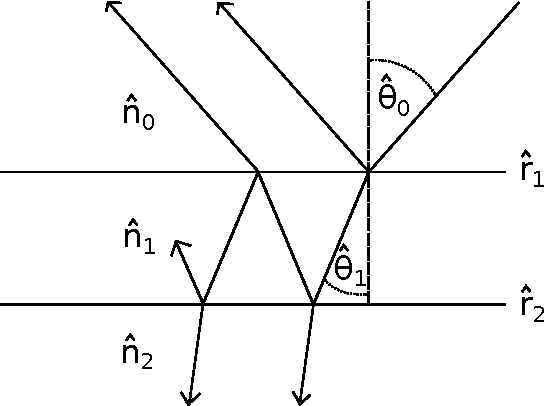
\includegraphics[width=13cm]{schema.pdf}
\caption{Schéma aparatury, K -- klystron, C -- cirkulátor, ZN -- zdroj napětí pro doutnavý výboj, HS -- Hallova sonda, $\alpha$ -- proměnlivý fázový člen, Z -- zapisovač}
\label{schema}
\end{center}
\end{figure}

\section{Měření}
\subsection{Zaznamenáme rezonanční křivky nejméně pro pět hodnot tlaku v rozmezí 100--2000\,Pa. Z jejich pološířek pak určíme závislost srážkové frekvence na tlaku.}

Rezonanční křivky byly zaznamenávány zapisovačem. Přímka pro převod z centimetrů na Tesla je na obrázku \ref{prevod}, její směrnice je $a = (4,16 \pm 0,09)10^{-3} \mathrm{ T/cm}$. 

\begin{figure}[!htbp]
\begin{center}
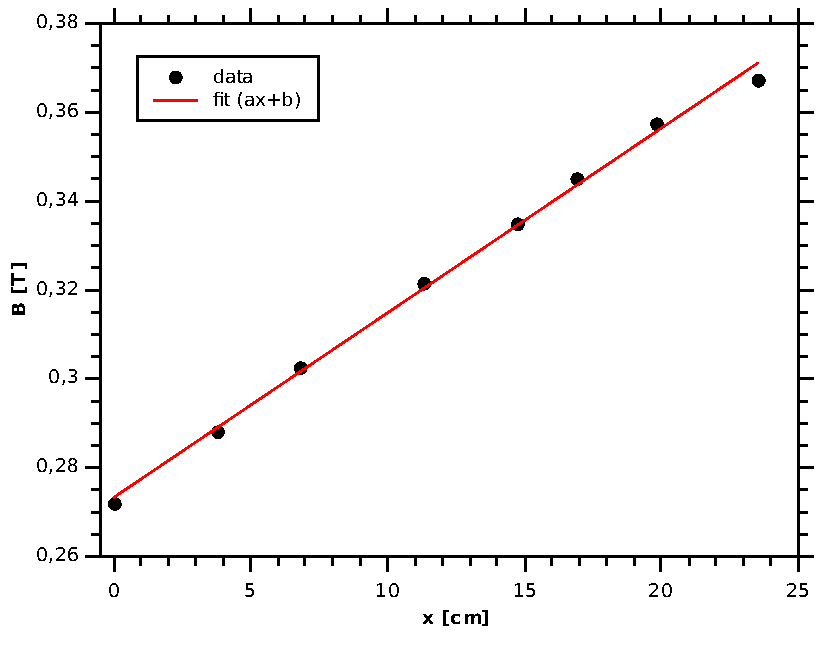
\includegraphics[width=12cm]{Graph2.pdf}
\caption{Kalibrační křivka pro převod.}
\label{prevod}
\end{center}
\end{figure}

Zároveň byla měřena i závislost intenzity magnetického pole na proudu elektromagnetem. Na obrázku \ref{magnet} můžeme vidět, že pro nízké proudy je závislost přibližně lineární, pro vyšší proudy už se elektromagnet začíná sytit.

\begin{figure}[!htbp]
\begin{center}
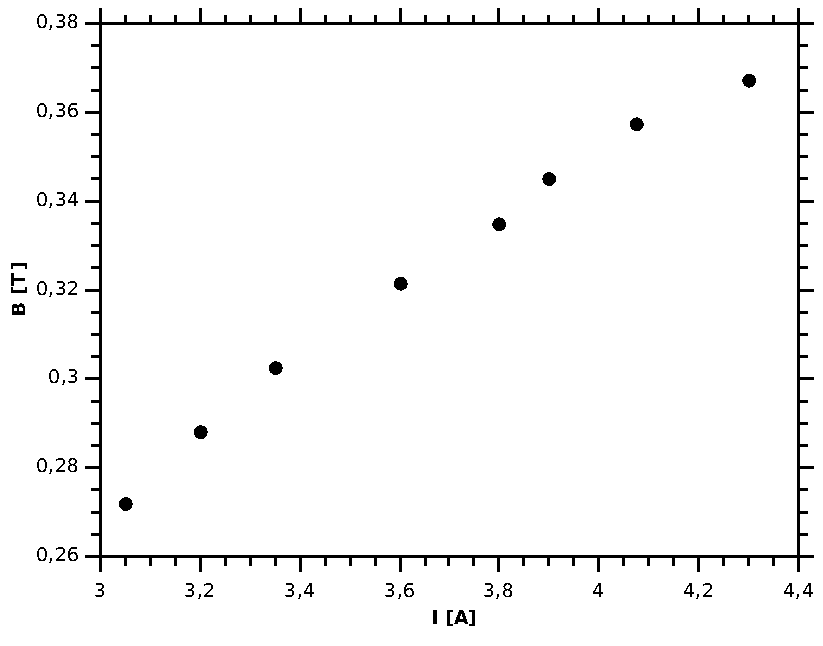
\includegraphics[width=12cm]{Graph1.pdf}
\caption{Intenzita magnetického pole v závislosti na proudu v elektromagnetu.}
\label{magnet}
\end{center}
\end{figure}

První měření bylo prováděno při konstantním výbojovém proudu  1\,mA a proměnném tlaku, výsledky jsou v tabulce \ref{t1} a na obrázku \ref{vnap}.

\begin{table}[htbp]
\begin{center}
\begin{tabular}{|c|c|c|c|}
\hline
$p$ [Pa] & Pološířka [cm] & Pološířka [mT] & $\nu [10^9 \mathrm{s}^{-1}]$ \\ \hline
100 & 3,35 & 13,94 & 2,45 \\ \hline
150 & 2,85 & 11,86 & 2,09 \\ \hline
200 & 2,4 & 9,98 & 1,76 \\ \hline
300 & 2,9 & 12,06 & 2,12 \\ \hline
400 & 3,75 & 15,62 & 2,74 \\ \hline
500 & 3,9 & 16,22 & 2,85 \\ \hline
\end{tabular}
\caption{Závislost srážkové frekvence na tlaku, viz obrázek \ref{vnap}}
\label{t1}
\end{center}
\end{table}

\begin{figure}[!htbp]
\begin{center}
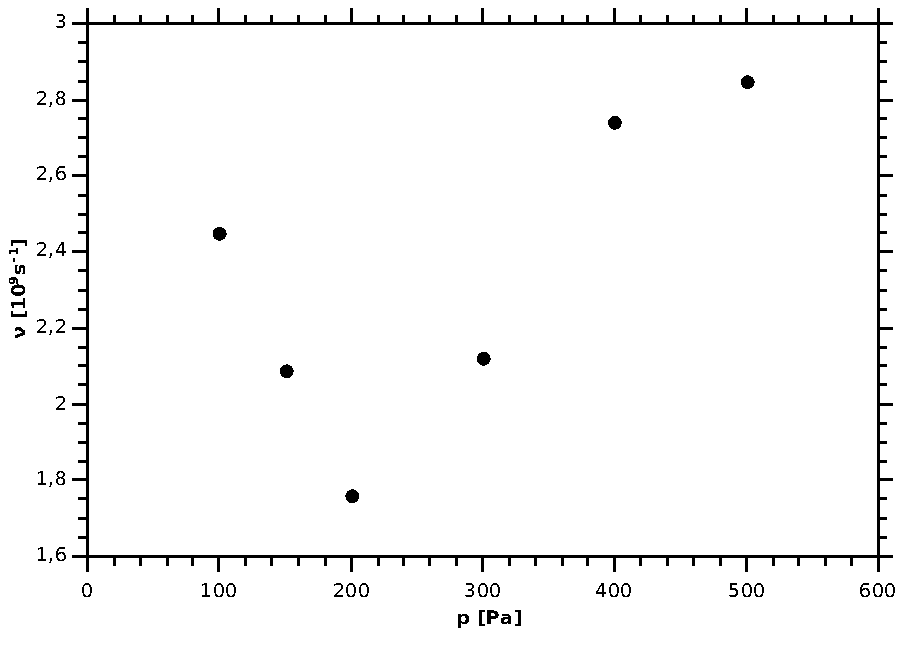
\includegraphics[width=12cm]{Graph3.pdf}
\caption{Závislost srážkové frekvence na tlaku}
\label{vnap}
\end{center}
\end{figure}

Další měření bylo prováděno při konstantním tlaku 100\,Pa a proměnném výbojovém proudu, výsledky jsou v tabulce \ref{t2} a na obrázku \ref{vnai}.

\begin{table}[htbp]
\begin{center}
\begin{tabular}{|c|c|c|c|}
\hline
$I$ [mA] & Pološířka [cm] & Pološířka [mT] & $\nu [10^9 \mathrm{s}^{-1}$] \\ \hline
0,14 & 0,95 & 3,95 & 0,69 \\ \hline
0,2 & 1,45 & 6,03 & 1,06 \\ \hline
0,3 & 1,6 & 6,66 & 1,17 \\ \hline
0,4 & 1,7 & 7,07 & 1,24 \\ \hline
0,5 & 2,1 & 8,74 & 1,54 \\ \hline
0,6 & 2,375 & 9,88 & 1,74 \\ \hline
0,7 & 2,675 & 11,13 & 1,96 \\ \hline
0,8 & 3 & 12,48 & 2,19 \\ \hline
0,9 & 3,25 & 13,52 & 2,38 \\ \hline
1 & 3,55 & 14,77 & 2,60 \\ \hline
\end{tabular}
\end{center}
\caption{Závislost srážkové frekvence na výbojovém proudu.}
\label{t2}
\end{table}

\begin{figure}[!htbp]
\begin{center}
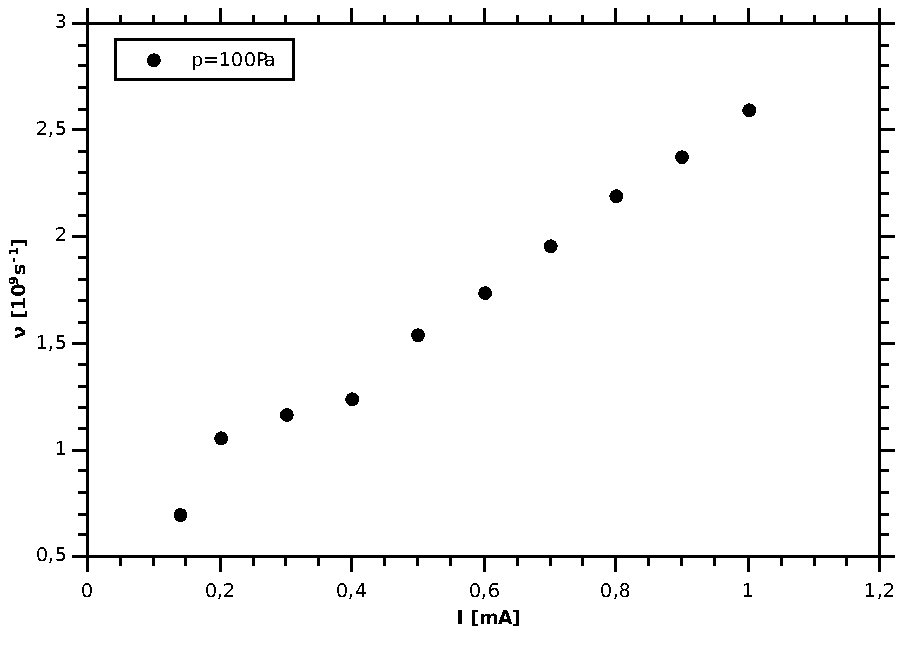
\includegraphics[width=12cm]{Graph4.pdf}
\caption{Závislost srážkové frekvence na výbojovém proudu.}
\label{vnai}
\end{center}
\end{figure}

\section{Závěr}
Měření proběhlo úspěšně. Podařilo se naměřit srážkovou frekvenci jak pro různé tlaky tak pro různé výbojové proudy. Ukázalo se že srážková frekvence s výbojovým proudem roste lineárně. V tlakové závislosti je vidět minimum přibližně na hodnotě 200\,Pa, ale na detailnější analýzu tvaru křivky bylo provedeno málo měření. Tyto výsledky se neshodují s teoretickým očekáváním, kdy při rostoucím tlaku bychom očekávali rostoucí srážkovou frekvenci (se vzrůstající koncentrací neutrálů klesá střední volná dráha), a naopak na výbojovém proudu by měla srážková frekvence záviset minimálně. Obě měřené závislosti se protínají pro 1\,mA a 100\,Pa, z čehož můžeme usoudit o opakovatelnosti měření. Pro hodnotu 100\,Pa a výbojový proud 1\,mA kde bylo měření prováděno dvakrát, se naměřené hodnoty liší přibližně o 5\,\%. Hlavní problémy při měření byly při odečítání z absorpčních píků, které byly často velmi nesymetrické (protáhlé doleva) a bylo také těžké určit jejich základnu, která byla na každé straně jinak.

\end{document}
